%!TEX root = ../template.tex
%%%%%%%%%%%%%%%%%%%%%%%%%%%%%%%%%%%%%%%%%%%%%%%%%%%%%%%%%%%%%%%%%%%%
%% chapter5.tex
%% NOVA thesis document file
%%
%% Chapter with lots of dummy text
%%%%%%%%%%%%%%%%%%%%%%%%%%%%%%%%%%%%%%%%%%%%%%%%%%%%%%%%%%%%%%%%%%%%
\chapter{Research Methodology}
\label{cha:methodology}

\section{Aimed contribution}%
\label{sec:aimed_contribution}

This work aims to answer its main \gls{RQ} by following and pursuing the
proposed hypothesis (see Section~\ref{sec:hypothesis_and_approach}). In
doing so, I will contribute with a commercially viable (from a technical
perspective) atmospheric monitoring system based on DOAS, capable of not
only measuring pollutant contamination but also mapping their
concentration in a given geographic region. This will generate several
intermediate steps, which are themselves smaller contributions:

The first intermediate step will be the development of a tomographic
strategy. This will of course include the selection of a sampling
geometry (consider the ones presented in
Section~\ref{sec:tomographic_algorithms_and_reconstruction_techniques}),
but also the positioning of "sources and sensors" within the selected
geometry. Since the system is designed to be a passive DOAS device (see
Section~\ref{sec:doas}), careful consideration must be taken in this
respect. Spectral acquisition must be done in a way that allows
tomographic reconstruction, but also respecting limitations and
particularities that come from working with solar light. This step
corresponds to answering the first secondary Research Question (see
Table~\ref{tab:sec_RQ}).

The next step will be to write a simulation tool for the tomographic
procedure. The idea is for this tool to encompass the acquisition
strategy that was defined in the previous step, in order to replicate
the whole measurement process and then perform the reconstruction using
one or more algorithms. The simulation tool has several functions. For
one, it allows the fine-tuning of the approaches without having to
expend any resources in purchasing material. Besides this, it also gives
gives researchers the chance to experiment with different algorithms.
The routine will be divided into two modules. The first module computes
the projections for a given phantom, and the second performs the
reconstruction with the projection data. The point is that one can write
a tomographic reconstruction routine and plug it to the projection
computation module, without any interference from one to the other. 

Finally we reach the instrumentation definition phase. In this stage, I
will have to select the optical components necessary to build this
system, including telescope, spectrometer and all the connection
components. In order to maintain this system as small as possible, I
will try to avoid using optical fibers, thus minimizing energy loss
between telescope and spectrometer. In this stage, I will also have to
design a mechanical support that allows a drone to be equipped with the
optical system, respecting all positioning and pointing requirements
that such a device must entail.

\section{Detailed work plan and scheduling}%
\label{sec:detailed_work_plan_and_scheduling}

In this section, I present the working plan for the proposed thesis. The
complete work plan is depicted in Figure~\ref{fig:low_res_gantt}. It
includes the 6 tasks, which take place in a period of 4 years of
research activities and scientific writing. The order in which the tasks
are performed is somewhat flexible (one could easily program the
trajectory (task 5) before conducting the experiments (task 3)), but the
presented sequence is the one that allows the best possible compromise
between scientific results and project accomplishment, taking into
account the hypothesis presented in
Section~\ref{sec:hypothesis_and_approach}.

\begin{figure}[htpb]
    \centering
    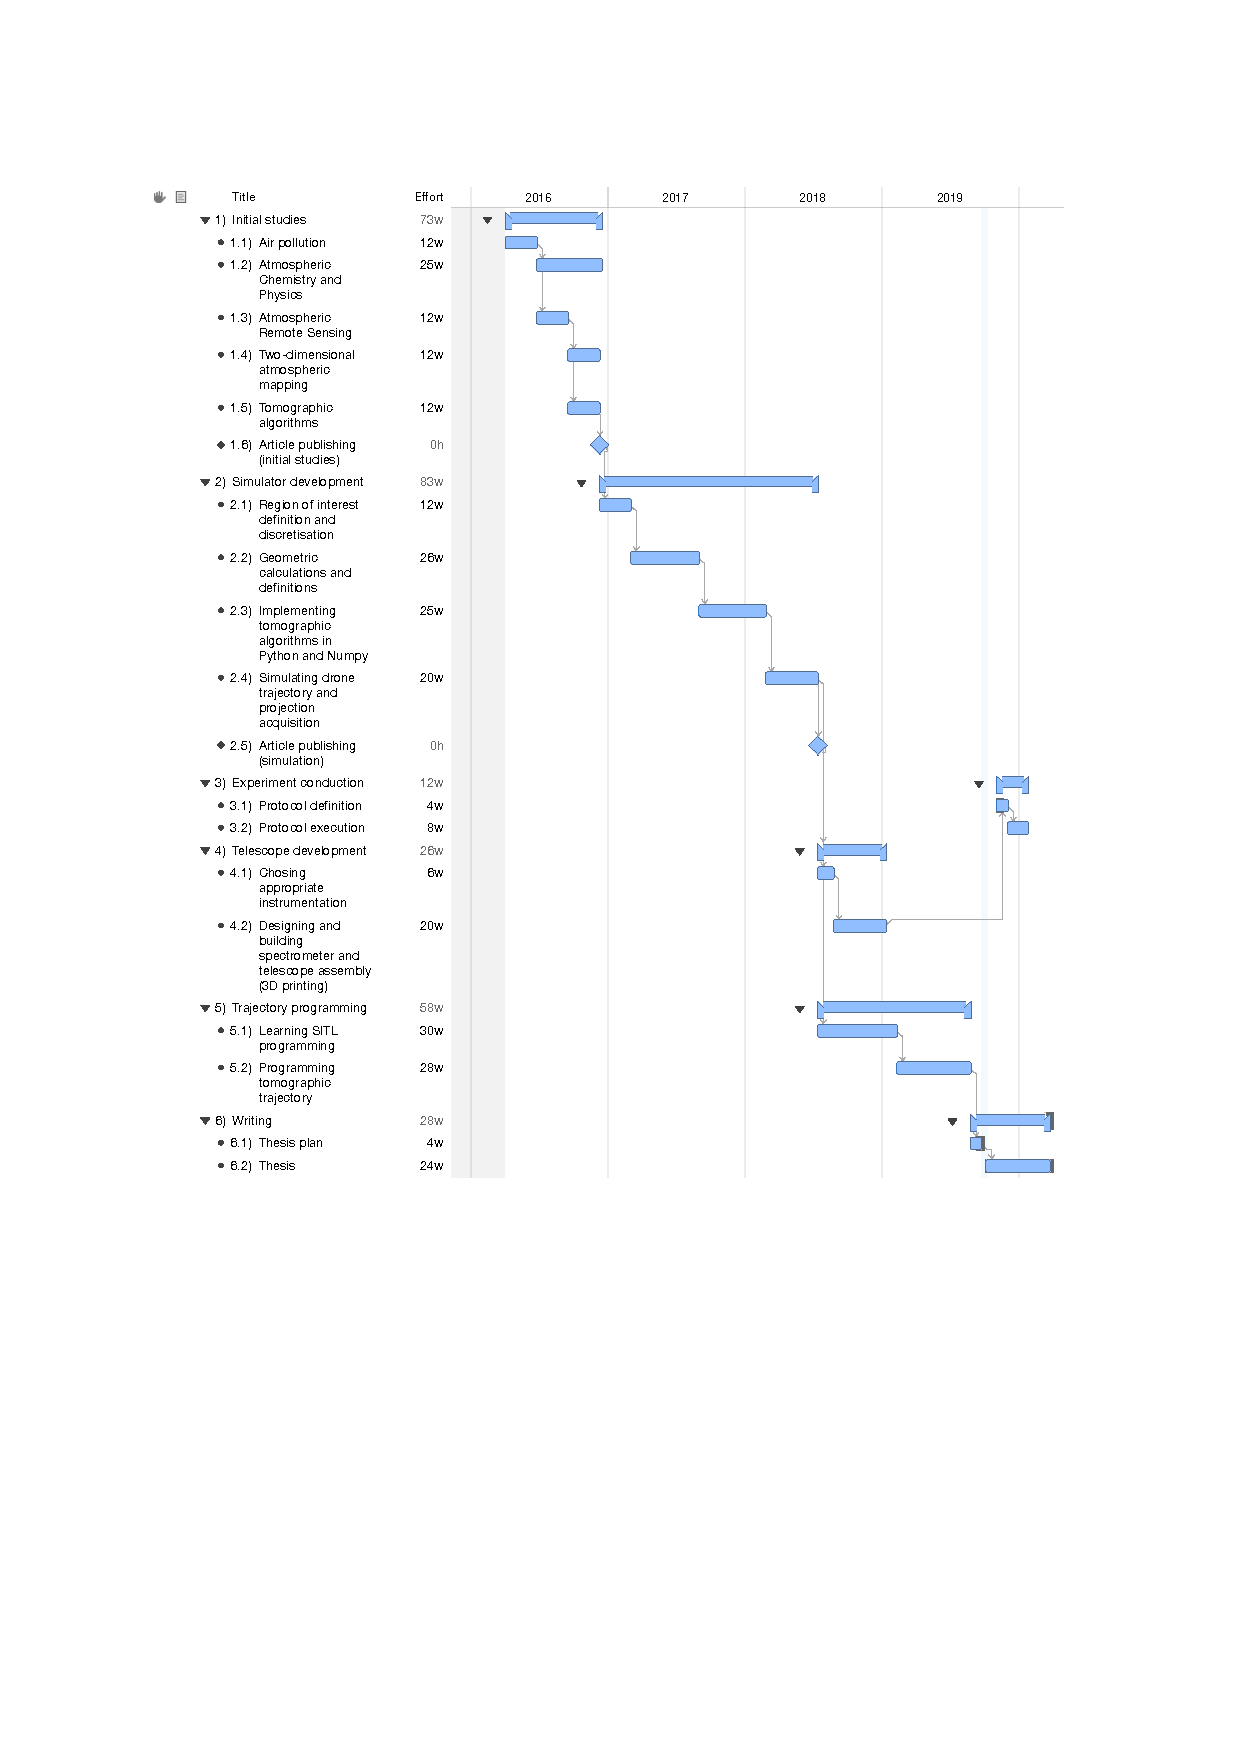
\includegraphics[width=0.8\textwidth]{img/gantt.pdf}
    \caption{Gantt chart for the proposed thesis. Note the main
    milestones in 2017 and 2019, which correspond to publication
    moments.}
    \label{fig:low_res_gantt}
\end{figure}

Task 1 is an exploratory task, in which I started reading the literature
in order to gain a good level of sensitivity to the subjects implied.
The task culminated in the writing of~\cite{ValentedeAlmeida2017} in
2017.

Task 2 encompassed the development of a simulation module for the
tomographic method with which I intended to retrieve a two-dimensional
concentration mapping for certain atmospheric trace gases. The module
includes a precise geometric description and error estimation (using
Monte Carlo methods) and intends to simulate the formation of a fan-beam
measurement using a specific circular trajectory. This task should
result in one publication.

The third task concerns experiment conduction. These experiments are
designed to verify the acquisition method hypothesis which was simulated
in Task 2. Conducting this task shall require developing the experiment
protocol as well as its final execution.

The spectral acquisition strategy for the proposed project involves the
development of an optical assembly without any fiber-optics. In task 4,
I shall choose the optical components for this assembly and design it
using 3D CAD methods. Finally, the assembly is to be manufactured: first
in a 3D printer and then using traditional metal milling methods.


\section{Validation methodology}%
\label{sec:validation_methodology}

There are several ways to validate a piece of work as the one I present
here. It is important to do this in more than one, to ensure not only
the validity of the project, but also its relevancy.

Before going any further, I should mention that although my project was
conducted as part of the pursuit of a doctoral degree, it was not a
traditional PhD, in the sense that it was not done solely in a
University setting. The grant that I was awarded by the Portuguese
Foundation for Science and Technology was part of a PhD Program for
degrees conducted in partnership between FCT NOVA and a group of
companies, named NOVA Instrumentation for Health (NOVA I4H). This is
relevant as it indicates that there is at least a commercial interest in
developing the technology I propose with this thesis (a market
validation of sorts). Otherwise, the project would not be viable for the
company.

One important way in which I will validate this project is by publishing
in significant peer reviewed publications. As illustrated in
Figure~\ref{fig:low_res_gantt}, during the course of my PhD, I intend to
publish two relevant articles in Web-of-Science-indexed publications.
The first of these was published in 2017, at the end of the preliminary
studies stage of the project. The second is currently in the finishing
stages of writing and should be submitted before the end of September.
Conference-wise, I plan to introduce my work to the scientific community
in 2020, by participating in at least one acknowledged conference in the
remote sensing or atmospheric monitoring community.
Table~\ref{tab:dissemination_plan} summarizes the project's
dissemination plan.

\begin{table}[htpb]
    \centering
    \caption{Dissemination plan for the PhD Project.}
    \label{tab:dissemination_plan}
    \begin{tabular}{c}
    
    \end{tabular}
\end{table}




\section{Integration with other research activities}%
\label{sec:integration_with_other_research_activities}

As stated in Chapter~\ref{cha:bg_and_motivation}, this project started
as a direct evolution from the Forest Fire Finder system, an autonomous
forest fire detection device. In 2017, NGNS-IS (the birthplace of
\gls{FFF}) was absorber by the Compta group, and \gls{FFF} became
Bee2Fire. As an extension to the Bee2Fire, this project is integrated in
Compta's research efforts, namely in the remote sensing and artificial
intelligence department. 

In addition to this, the present work is supported by the Portuguese
Foundation for Science and Technology, through the NOVA I4H PhD Program
(grant reference: PDE/BDE/114549/2016).






